\documentclass[11pt]{article}

\usepackage{geometry}
\geometry{a4paper}

\usepackage{graphicx}
\usepackage{amssymb}
\usepackage{physics}
\usepackage{amsmath}
\usepackage{lipsum}

\usepackage{cite} %Uses proper indexing when citing multiple papers
\usepackage{authblk} %Shows all authors with e-mail addresses and affiliations properly on the page

%%%%%%%%%%%%%%%%%%%%%%%%%%%%%%% INFO %%%%%%%%%%%%%%%%%%%%%%%%%%%%%%%%%%%%%%%%%
\title{Extensive Study of the Wobbling Properties in $^{163}$Lu for the Positive and Negative Parity States} 

\author[1,2]{Robert Poenaru \thanks{E-mail: robert.poenaru@drd.unibuc.ro}}
\author[2,3]{Apolodor Aristotel Raduta \thanks{E-mail: raduta@nipne.ro}}

\affil[1]{Doctoral School of Physics, University of Bucharest, Romania}
\affil[2]{\textit{Horia Hulubei} National Institute for Physics and Nuclear Engineering, M\u{a}gurele-Bucharest, Romania}
\affil[3]{Academy of Romanian Scientists, Bucharest, Romania}
%%%%%%%%%%%%%%%%%%%%%%%%%%%%%%% INFO %%%%%%%%%%%%%%%%%%%%%%%%%%%%%%%%%%%%%%%%%

\date{\today}

\begin{document}

\bibliographystyle{unsrt}

\maketitle

%%%%%%%%%%%%%%%%%%%%%%%%%%%%%%% TEXT %%%%%%%%%%%%%%%%%%%%%%%%%%%%%%%%%%%%%%%%%
\begin{abstract}
A new interpretation on the wobbling structure in $^{163}$Lu is developed, based on the concept of parity symmetry. It is known that four wobbling bands are experimentally observed in this isotope, where three of them are considered as wobbling phonon excitations (namely $TSD_2$, $TSD_3$, and $TSD_4$) and the yrast band for the ground state (that is TSD1). In the present work, the trial function that is used for obtaining the wobbling spectrum is analyzed in terms of its behavior under the rotation operation. Indeed, due to a specific symmetry to rotations with $\pi$ around the 2-axis of the triaxial system, the parity becomes a good quantum number. As such, the trial function admits solutions with negative parity, which belong to the rotational states in $TSD_4$. A unified description of all the triaxial super-deformed bands in $^{163}$Lu is achieved with the new formalism.
\end{abstract}

\section{Introduction}

Triaxiality in nuclei has become an interesting topic for physicists over the years, mainly due to its great challenge of measure it experimentally, but also for its large number of characteristics that are said to be resulting from these kind of shapes. Moreover, stable triaxial shapes are of rare occurrence across the chart of nuclides \cite{moller2006global}, since the predominant character of nuclei is either spherical or axially symmetric. Over the last two decades, it has been shown that triaxiality plays a crucial role in measurements of important quantities like proton emission probabilities \cite{delion2006theories}, separation energies of the nucleons \cite{moller2006global}, and also fission barriers in heavy nuclei  \cite{moller2009heavy}, however, concrete evidences of triaxiality in nuclei were still missing or under investigation. A tremendous work was given in finding a clear signature for non-axially symmetric shapes: effects such as anomalous signature splitting \cite{hamamoto1988triaxial}, signature inversion \cite{bengtsson1984signature}, and staggering of $\gamma$ bands \cite{stachel1982triaxiality} were pointed, but only recently two clear fingerprints of nuclear triaxiality have emerged in the literature, based on both experimental and theoretical findings. Indeed, the phenomena of \emph{chiral symmetry breaking} and that of \emph{wobbling motion} (W.M.) are considered as unique characteristics of nuclear triaxiality. 

Chirality consists in the existence of a pair of chiral twin bands with an identical structure and almost similar energies. These bands are expected to appear due to the coupling of valence nucleons and the collective mode of rotation that could drive the total spin away from any of the three principal planes, giving rise to both left-handed and right-handed orientation of the angular momentum vectors \cite{frauendorf1997tilted}. A rigorous investigation of all the nuclei with chiral bands is given by Xiong and Wang in \cite{xiong2019nuclear}, where reportedly a total of 59 chiral doublet bands in 47 such nuclei are confirmed. As a matter of fact, 8 of these nuclei have multiple chiral doublets. 

On the other hand, the experimental observations regarding wobbling motion have been quite rare, even though this kind of collective motion has been theoretically predicted almost 50 years ago by Bohr and Mottelson \cite{bohr1998nuclear} when they were investigating the rotational modes of a triaxial nucleus by means of a Triaxial Rotor Model (TRM). Therein, they showed that for a triaxial rotor, the main rotational motion is around the axis with the largest moment of inertia (MOI), as it is energetically the most favorable. This mode is quantum mechanically disturbed by the rotation around the other two axes, since rotation around any of the three principal axes of the system are possible, due to the anisotropy of the three different MOIs (that is $\mathcal{I}_1\neq\mathcal{I}_2\neq\mathcal{I}_3$).

W.M. can be viewed as the quantum analogue to the motion of the asymmetric top, whose rotation around the axis with largest MOI is energetically favored and stable. A uniform rotation about this axis will have the lowest energy for a given angular momentum (spin). As the energy increases, this axis will start to precess with a harmonic type of oscillation about the space-fixed angular momentum vector, giving rise to a family of wobbling bands, each characterized by a wobbling phonon number $n_w$. The resulting quantal spectrum will be a sequence of rotational $\Delta I=2$ bands, with alternating signature number for each wobbling excitation. According to \cite{bohr1998nuclear}, it is possible to obtain the wobbling spectrum of any triaxial rigid rotor, by using the information related to its angular momentum $I$, moments of inertia $\mathcal{I}_{1,2,3}$, rotational frequency $\omega_\text{rot}$, wobbling frequency $\omega_\text{wob}$ as follows:

\begin{align}
    E_\text{rot}=\sum_i\left(\frac{\hbar^2}{2\mathcal{I}_k}\right)I^2_k\approx\frac{\hbar^2}{2\mathcal{I}_1}I(I+1)+\hbar\omega_\text{wob}\left(n_w+\frac{1}{2}\right)\ , \label{wobbling_eq}
\end{align}

with $\omega_\text{wob}$ given by the following expression:
\begin{align}
    \hbar\omega_\text{wob}=\hbar\omega_\text{rot}\sqrt{\frac{(\mathcal{I}_x-\mathcal{I}_y)(\mathcal{I}_x-\mathcal{I}_z)}{\mathcal{I}_y\mathcal{I}_z}}\ .
\end{align}

where the rotational frequency of the rigid rotor is given by $\hbar\omega_\text{rot}=\frac{\hbar I^2}{\mathcal{I}_1}$. In Eq. \ref{wobbling_eq}, the approximation of very large MOI along 1-axis is considered (i.e., $\mathcal{I}_1>>\mathcal{I}_2,\mathcal{I}_3$), and $I(I+1)=I_x^2+I_y^2+I_z^2$. One can see that the wobbling motion is expressed as a 1-dimensional vibration with only one variable, since the energy of the zero-point fluctuation is $\frac{\hbar\omega_\text{wob}}{2}$ \cite{hagemann2003quantized}.

Just for an illustrative purpose, Figure \ref{simple-wobbling-family} shows a theoretical spectrum for the wobbling bands within a triaxial rigid rotor. The family of wobbling bands are obtained from a set of three moments of inertia (along the three principal axes), a given angular momentum, and different wobbling phonon numbers. Moreover, in Figure \ref{simple-wobbling-family}, the tilting of the angular momentum away from the rotational axis is sketched, where the tilt increases with the increase in the wobbling excitation.

\begin{figure}
\centering
\begin{minipage}{.6\textwidth}
  \centering
  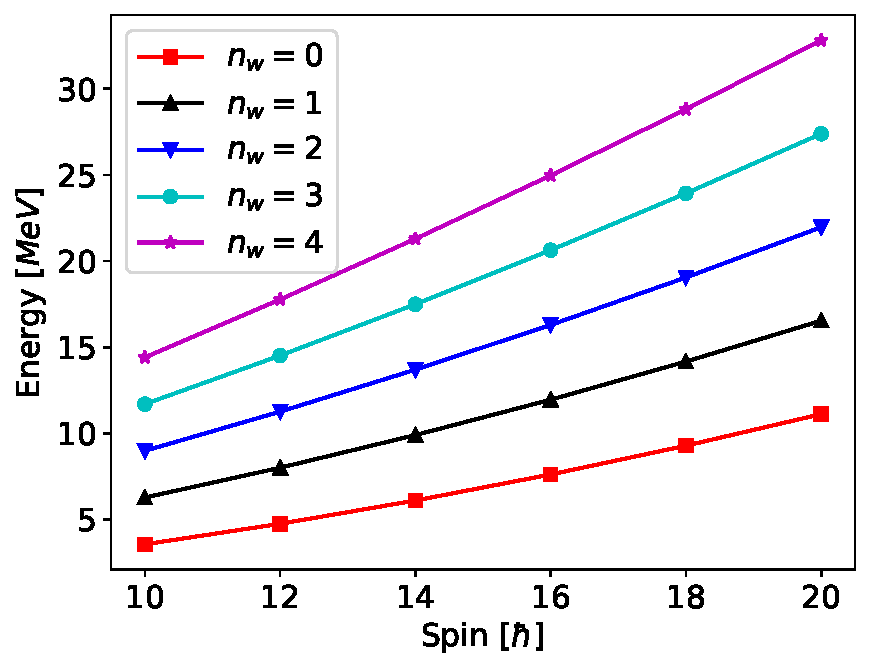
\includegraphics[width=1\linewidth]{figs/simple_wobbling_spectrum.pdf}
  %  \caption{A family of wobbling bands for a triaxial rigid rotor (schematic representation). The calculations were done for $\mathcal{I}_1:\mathcal{I}_2:\mathcal{I}_3=25:5:2$.}
    % \label{simple-wobbling-family}
\end{minipage}%
\begin{minipage}{.4\textwidth}
  \centering
 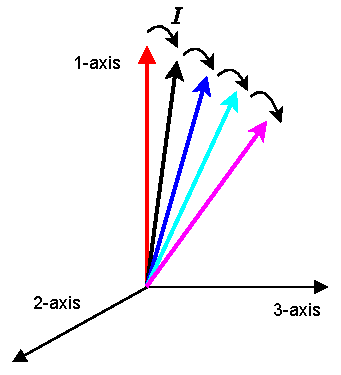
\includegraphics[width=0.8\linewidth]{figs/wobbling_tilting_axis.pdf}
   % \caption{Tilting of the angular momentum away from the rotational axis, with increase in the wobbling phonon excitation.}
    % \label{wobbling-tilt}
\end{minipage}
\label{simple-wobbling-family}
\caption{Family of wobbling bands for a simple triaxial rotor (left-side). Tilting of the angular momentum vector away from the rotational axis (right-side). This schematic representation was done for an arbitrary set of MOIs $\mathcal{I}_1:\mathcal{I}_2:\mathcal{I}_3=25:5:2$.}
\end{figure}


\section{Theoretical Background}

The Hamiltonian of the system is given in terms of a term that corresponds to the core deformation, and a second term which corresponds to the valence nucleon moving in a mean-field with quadrupole character (generated by the triaxial core).

\begin{align}
    \hat{H}=\hat{H}_\text{rot}+\hat{H}_\text{s.p.}.
\end{align}

%%%%%%%%%%%%%%%%%%%%%%%%%%%%%%% TEXT  %%%%%%%%%%%%%%%%%%%%%%%%%%%%%%%%%%%%%%%%%

\bibliography{references}

\end{document}  